



\documentclass[11pt,a4paper]{scrartcl}
\typearea{12}
\usepackage{graphicx}
\usepackage{amsmath}
\usepackage{listings}
\usepackage{color}
\usepackage{tikz}
\usetikzlibrary{decorations.markings}
\lstset{language=C}
\usepackage{fancyhdr}
\pagestyle{fancy}
\begin{document}




\section*{Worksheet 8 - copied from Martha Lewis}

\subsection*{Q1}
$X$ and $Y$ are two (binary) random variables. If $X$ and $Y$ are independent, then:
\begin{equation}
    P(X, Y) = P(X)P(Y)
\end{equation}

\begin{enumerate}
\item Give an example of two random variables that are independent.

\item Complete the probability table below in such a way that the variables $X$ and $Y$ are independent.

\begin{center}
    \begin{tabular}{c|cc}
        & $X = 0$ & $X = 1$ \\
        \hline
        $Y = 0$ & $?$ & $? $\\
        $Y = 1$ & $?$ & $? $
    \end{tabular}
\end{center}


\item Determine the missing entries $(a, b)$ of the joint distribution in such a way that the variables $X$ and $Y$ are again independent:
\begin{align*}
    P(Y = 0, X = 0) &= 0.1 \\
    P(Y = 0, X = 1) &= 0.3 \\
    P(Y = 1, X = 0) &= a \\
    P(Y = 1, X = 1) &= b
\end{align*}
\end{enumerate}

\subsection*{Q2}
Exactly a fifth of the people in a town have lycanthropy. There
  are two tests for lycanthropy, ASSAY1 and ASSAY2. When a person goes
  to a doctor to test for lycanthropy, with probability 2/3 the doctor
  conducts ASSAY1 on them and with probability 1/3 the doctor conducts
  ASSAY2 on them. When ASSAY1 is done on a person, the outcome is as
  follows: If the person has the disease, the result is positive with
  probability 3/4. If the person does not have the disease, the result
  is positive with probability 1/4. When ASSAY2 is done on a person,
  the outcome is as follows: If the person has the disease, the result
  is positive with probability 1. If the person does not have the
  disease, the result is positive with probability 1/2. A person is
  picked uniformly at random from the town and is sent to a doctor to
  test for lycanthropy. The result comes out positive. What is the
  probability that the person has the disease?\footnote{Taken from
  allendowney.blogspot.com/2017/02/a-nice-bayes-theorem-problem-medical.html}

\subsection*{Q3}
Consider the following Bayesian network:

\begin{center}
    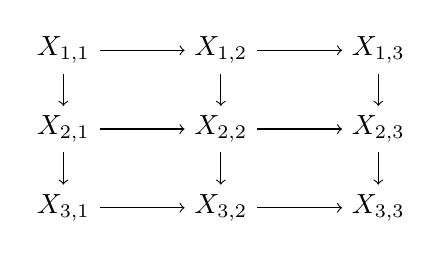
\begin{tikzpicture}
        \node (X11) at (0,2) {$X_{1,1}$};
        \node (X12) at (2,2) {$X_{1,2}$};
        \node (X13) at (4,2) {$X_{1,3}$};
        \node (X21) at (0,1) {$X_{2,1}$};
        \node (X22) at (2,1) {$X_{2,2}$};
        \node (X23) at (4,1) {$X_{2,3}$};
        \node (X31) at (0,0) {$X_{3,1}$};
        \node (X32) at (2,0) {$X_{3,2}$};
        \node (X33) at (4,0) {$X_{3,3}$};

        \draw[->] (X11) -- (X12);
        \draw[->] (X12) -- (X13);
        \draw[->] (X11) -- (X21);
        \draw[->] (X12) -- (X22);
        \draw[->] (X13) -- (X23);
        \draw[->] (X21) -- (X31);
        \draw[->] (X22) -- (X32);
        \draw[->] (X23) -- (X33);
        \draw[->] (X21) -- (X22);
        \draw[->] (X22) -- (X23);
        \draw[->] (X31) -- (X32);
        \draw[->] (X32) -- (X33);
    \end{tikzpicture}
\end{center}

(a) Which random variables are independent of $X_{3,1}$?

(b) Which random variables are independent of $X_{3,1}$ given $X_{1,1}$?

\end{document}
